\chapter{Exercises 4}

\section{Short problems}

\textbf{\\Problem 2 \\
Assume Alice has two databases: a trusted storage (that an
attacker cannot read and modify), and an \textcolor{Red}{untrusted storage}
(that an attacker can read and modify). Assume Alice can
use:
\begin{itemize}
    \item H : a secure cryptographic hash function, like SHA256
    \item || : the concatenation function 
\end{itemize}
Alice creates and stores four files, F1, F2, F3, F4 in the
\textcolor{Red}{untrusted storage}. Alice also computes and stores a hash of
each file (content) in the \textcolor{Red}{untrusted storage}:
h1 = H(F1), h2 = H(F2), h3 = H(F3), h4 = H(F4)
Then, Alice calculates hchain and stores it in the \textcolor{Blue}{trusted storage}:
hchain = H( h1 || h2 || h3 || h4 )
Let's assume Bob modifies F3.}

\textbf{\\P2Q - Can Alice detect the modification done by Bob?}
\begin{itemize}
    \item[A.] Yes, Alice recomputes h3 = H(F3) and sees that it doesn't match with the stored h3
    \item[B.] \sol{Yes, Alice recomputes $h_{chain}$ and sees that it doesn't match with the stored $h_{chain}$}
    \item[C.] No, Alice cannot detect the modification because the attacker can change both F3 and H(F3)
\end{itemize}
\com{
    A -> the h3 stored could be manipulated too\\
    C -> if h3 change, $h_{chain}$ will fail the match, so we can  detect it}

\textbf{\\Problem 3 \\
Assume Alice has one \textcolor{Blue}{trusted storage} (that an attacker cannot
read and modify), and an \textcolor{Red}{untrusted storage} (that an attacker
can read and modify). Assume Alice can use two functions:
\begin{itemize}
    \item H, a secure cryptographic hash function, like SHA256
    \item || , the concatenation function
\end{itemize}
Alice creates and stores four files (F1, F2, F3, F4) in the
\textcolor{Red}{untrusted storage}. Alice also computes a hash on each file
(content):
h1 = H(F1), h2 = H(F2), h3 = H(F3), h4 = H(F4)
Then, Alice calculates $h_{root}$ and stores it the \textcolor{Blue}{trusted storage}:
$h_{root} = H(H(h1||h2)||H(h3||h4))$
Let's assume Bob modifies F3.}

\textbf{\\P3Q - Can Alice detect the modification done by Bob?}
\begin{itemize}
    \item[A.] Yes, Alice recomputes h3 = H(F3) and sees that it doesn't match with the stored h3
    \item[B.] \sol{Yes, Alice recomputes $h_{root}$ and sees that it doesn't match with the stored $h_{root}$}
    \item[C.] No, Alice cannot detect the modification because the attacker can change both F3 and H(F3)
\end{itemize}
\com{the change propagetes through all the tree}

\section{Security of IP networks}
\textbf{\\Q1 - Which protocol can be exploited for user authentication in dial-up, wireless, or virtual links (you can select multiple choices)?}
\begin{itemize}
    \item[A.] RADIUS
    \item[B.] \sol{EAP}
    \item[C.] DIAMETER
    \item[D.] \sol{CHAP}
\end{itemize}
\com{
    Authentication of PPP channel\\
    A -> Remote Authentication Dial-In User Service \\
    B -> Extensible Authentication Protocol\\
    C -> evoulition of RADIUS
    D -> Challenge Handshake Authentication Protocol 
}

\textbf{\\Q2 - At which level in the OSI stack is EAP (Extensible Authentication Protocol) exploited to support authentication?}
\begin{itemize}
    \item[A.] \sol{L2 (data link layer)}
    \item[B.] L3 (network level)
    \item[C.] L7 (application level)
    \item[D.] L4 (transport level)
\end{itemize}
\com{it support PPP and other L2 protocol }

\textbf{\\Q3 - Assume that we have a small company which uses a NAS supporting EAP, PAP, CHAP. Look at the picture and tell which methods and protocol(s) can be used to authenticate a user (device) with the NAS to provide it access to Internet:}
\begin{itemize}
    \item[A.] RADIUS
    \item[B.] \sol{PAP}
    \item[C.] \sol{CHAP}
\end{itemize}
\begin{figure}[h]
    \centering
    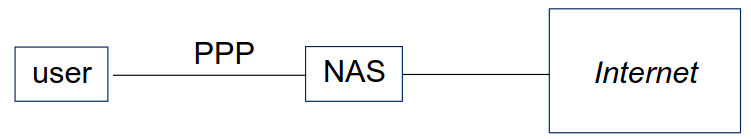
\includegraphics[width = 0.70\textwidth]{exercises4/question3.png}
\end{figure}
\com{ authentication to the NAS  }

\textbf{\\Q4 - Assume we have a small hotel that uses an Access Point (NAS) supporting EAP, CHAP. Take a look at the picture below and indicate which methods can be used to authenticate a user (device) with the AP to provide access to the Internet:}
\begin{itemize}
    \item[A.] \sol{EAP-TLS}
    \item[B.] CHAP
    \item[C.] \sol{Username and password and EAP}
    \item[D.] RADIUS
    \item[E.] None of the above
\end{itemize}
\begin{figure}[h]
    \centering
    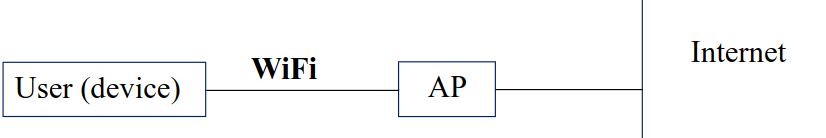
\includegraphics[width = 0.70\textwidth]{exercises4/question4.png}
\end{figure}
\com{(I'm not sure but->) CHAP this time is not used because in a hotel because of the computational work }

\textbf{\\Q5 - EAP transports authentication messages between a user (supplicant) and a NAS:}
\begin{itemize}
    \item[A.] \sol{before the IP channel is established. Thus, EAP uses its own encapsulation protocol because IP packets are not available}
    \item[B.] after the IP channel is established. Thus, EAP packets are encapsulated inside IP packets
    \item[C.] None of the above
\end{itemize}
\com{EAP (Extensible Authentication Protocol ) is the PPP authentication mechanism defined in RFC-
3748, providing a flexible Layer 2 (L2) authentication framework. This L2 authentication
occurs before accessing the internet, which operates at Layer 3 (L3)}

\textbf{\\Q6 - EAP can transport authentication messages between a user and NAS (Network Access Server):}
\begin{itemize}
    \item[A.] only for PPP channels
    \item[B.] \sol{for any L2 protocol, such as PPP, 802.11 (Wi-Fi), 802.3 (Ethernet), 802.5 (token ring)}
    \item[C.] only for 802.11 (Wi-Fi) and 802.3 (Ethernet)
\end{itemize}
\com{}



\textbf{\\Q7 - What is an EAP method (e.g. EAP-TLS, EAP-TTLS, EAP-SRP, AKA-SIM)?}
\begin{itemize}
    \item[A.] it's a variant to allow EAP to be exploited in other (upper level) protocols
    \item[B.] it's the method used by EAP to perform user authentication
    \item[C.] \sol{it's the method used by EAP to transfer the messages of a specific (user) authentication protocol}
    \item[D.] none of the above
\end{itemize}
\com{}

\textbf{\\Q8 - RADIUS is a network authentication protocol that:}
\begin{itemize}
    \item[A.] is used for communication (client-server schema) between a user (supplicant) and a NAS
    \item[B.] \sol{is used for communication (client-server schema) between a NAS and a backend Authentication Server (AS)}
    \item[C.] \sol{supports user authentication via PAP, CHAP, and EAP}
    \item[D.] supports user authentication only via EAP
    \item[E.] \sol{may act as a proxy towards other AS}
\end{itemize}
\com{This question should help you understand previous questions about NAS. }

\textbf{\\Q9 - Assume we have a corporate network which has an Authentication Server (AS) in place, and uses an AP for network access control. 
Take a look at the picture below and indicate the protocol(s) typically used for the communication between AP and AS during authentication of supplicants:}
\begin{itemize}
    \item[A.] \sol{RADIUS}
    \item[B.] PAP
    \item[C.] CHAP
\end{itemize}
\begin{figure}[h]
    \centering
    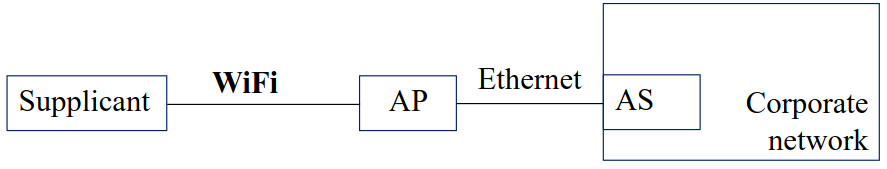
\includegraphics[width = 0.70\textwidth]{exercises4/question9.png}
\end{figure}
\com{}


\textbf{\\Q10 - RADIUS implements the following security properties:}
\begin{itemize}
    \item[A.] authentication and integrity of requests, where the RADIUS requests are protected with a digital signature
    \item[B.] \sol{authentication and integrity of requests, where the RADIUS requests are protected with a keyed-digest}
    \item[C.] authentication and integrity of responses, where the RADIUS responses are digitally signed by the RADIUS server
    \item[D.] \sol{authentication and integrity of responses, where the RADIUS responses are protected with a keyed-digest}
    \item[E.] authentication of the server, through the calculation of an authenticator via keyed-digest
\end{itemize}
\com{wip}

\textbf{\\Q11 - RADIUS implements the following security properties:}
\begin{itemize}
    \item[A.] confidentiality of the data in the RADIUS request by encrypting the data with an algorithm that can be negotiated
    \item[B.] \sol{confidentiality of the data in the RADIUS request by masking the (user) password (with an XOR operation)}
    \item[C.] confidentiality of the data in the RADIUS response by encrypting the data with an algorithm that can be negotiated
    \item[D.] confidentiality of the data in the RADIUS response by masking the password (with an XOR operation)
    \item[E.] protection from replay of RADIUS response, by using a sequence number in the RADIUS response
    \textbf{\item[F.] protection from replay of RADIUS response, by binding the response to a specific request via a Request Authenticator}
\end{itemize}
\com{wip}

\textbf{\\Q12 - Consider an architecture in which we have: a supplicant (user), a NAS, and a RADIUS server. If the
RADIUS server and the user have a shared secret (named “secret”), does this mean that a (malicious) user can create
a fake RADIUS response?}
\begin{itemize}
    \item[A.] yes, because the user knows the secret
    \item[B.] no, because in the construction of the RADIUS response it is used also a Request Authenticator generated by the NAS
    \item[C.] \sol{no, because NAS and the RADIUS server have also a “secret” that the user does not know (used in protecting the RADIUS response)}
\end{itemize}
\com{wip}

\textbf{\\Q13 - Assume a company uses RADIUS to authenticate users and Wi-Fi access-points and switches enabled with support
for 802.1x. What is the main role of the Wi-Fi access points and switches and what needs to be done to allow them to
work when new user authentication protocols appear (and are supported by EAP)?}
\begin{itemize}
    \item[A.] \sol{allow to perform authentication of the users connecting to the AP or switch by exploiting EAP}
    \item[B.] \sol{encapsulate the EAP messages received from the users (supplicant) into RADIUS messages sent to the AS}
    \item[C.] must be updated if new user authentication protocols appear and are supported by EAP
    \item[D.] \sol{no change is needed if new user authentication protocols appear and are supported by EAP}
\end{itemize}
\com{wip}


